\TODO{articles about viewing interface,
constraints
and getting user input,
add smart sketchpad image,
end Navigation}
% group articles by domain 
% for every article write a short summary of its relevant features
% and add an illustrative picture
% then criticize the presented solutions

\subsection{Viewing Interface}
In order to obtain an immersive experience, there's a number of hardware
setups commonly available:

\begin{description}
	\item[Head Mounted Display (HMD)] --
	  Head mounting displays are glass shaped devices, projecting a pair of stereo
	  transformed images to the user's retinas.
	  They normally feature a gyroscope or similar apparatus to measure head orientation and tilt.
	  There are two kinds of HMDs: in the former the images are projected in small opaque screens;
	  in the latter the projected surface is translucid, allowing blending of real and virtual worlds.
	  
		Using a head mounted display has the benefit of sticking to the user's head
		and detecting head orientation.
		On the other hand each HMD serves one single user.
		Additionally, most users report suffering from fatigue after long periods of
		usage and it has limited resolution.
			
	\item[Cave Automatic Virtual Environment (CAVE)] --
	  A CAVE is an immersive virtual reality environment where projectors are directed to four,
	  five or all the six walls of a room-sized cube.
	  
		It shares the benefit of enclosing the user's viewing area with HMDs.
		Has a better resolution though.
		The downside is the small number of simultaneous users who can experience the CAVE at the same time.
	
	\item[Wall] --
	  A wall is a large surface, usually planar, filled by an image.
	  The whole image projection is responsibility of a cluster of projectors set up in a wall.
	  Each projector renders part of the surface and the border between projections is ideally minimal.
	  Each projector is controlled by an independent computer.
	  
		Its size and resolution depend entirely on the setup, but normally a wall offers high resolution
		(depends on the number of projectors in the grid and each projector's resolution).
		Due to the large surface of the wall, several users may be served as once.
		The downside is users having to face the wall to experience the image entirely.
\end{description}

\begin{figure}[!ht]
	\centering
	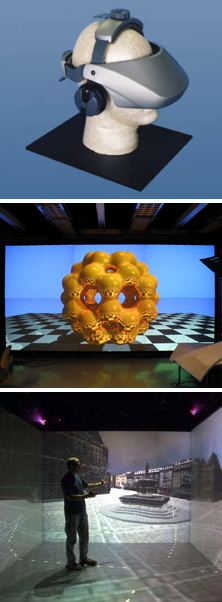
\includegraphics[width=11cm]{gfx/hmd-cluster-cave.png}
	\caption{HMD, Wall, CAVE}
	\label{FIG-HMD-CLUSTER-CAVE}
\end{figure}

Any of these setups is suitable for single user interaction.
In case of a reviewing session, in which at least two participants are required,
CAVE or Wall are better suited, since they alone offer a solution for a small group.

Using a Wall or CAVE presents other challenges: the computers responsible for
generating each projectors' images must be synchronized, its' color parameters calibrated,
the viewport must be well cropped, etc.
Several systems exist capable of delivering high performance 3D graphics and
offering the features mentioned above.
Based on scene graphs there are two well known solutions: OpenSceneGraph and OpenSG.

\subsection{Representing Urban Scenery}

How to effectively render city landscape.
One has to limit the detail of objects further away.
Ideally the transition should be smooth but recognizing each building's main shape
even far away is equally relevant.
This can be achieved implementing a solution like the following.

\subsubsection{Continuous LOD}
J�rgen D�llner and Henrik Buchholz \cite{LODCITY05} present a
solution for modeling buildings that feature a continuous level of detail.

The authors propose the following levels of detail for a building (derived from
CityGML\footnote{CityGML is a common information model for the representation of 3D urban objects.
It defines the classes and relations for the most relevant topographic objects in cities
and regional models with respect to their geometrical, topological, semantical and appearance properties.
More info at: http://www.citygml.org}, see Fig.\ref{FIG-LODCITY}):

\begin{itemize}
	\item Simple block model
	\item Model with defined roof geometry
	\item Detailed indoor and outdoor building features
\end{itemize}

\begin{figure}[!ht]
	\centering
	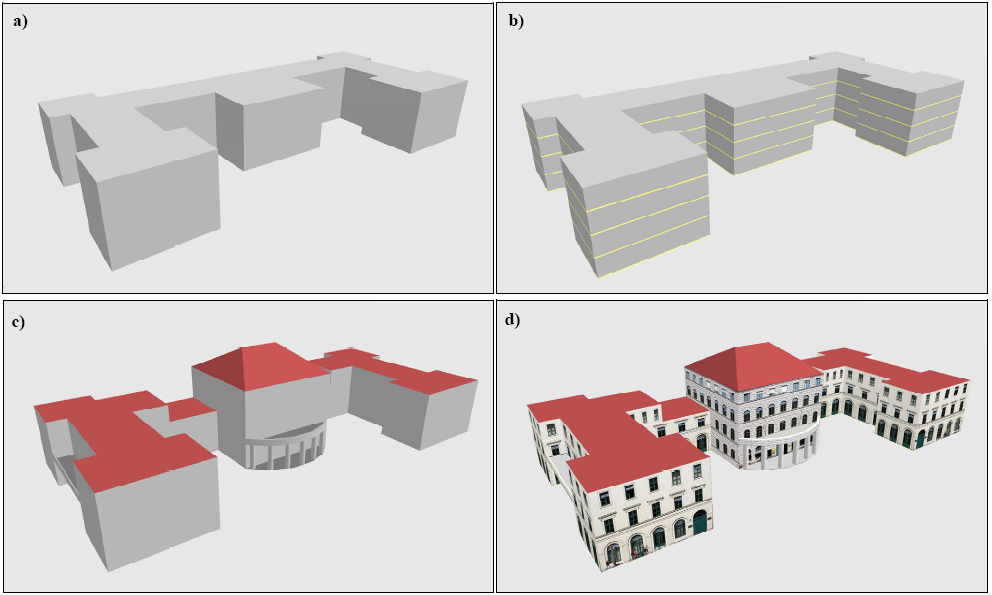
\includegraphics[width=11cm]{gfx/lodcity05-1.png}
	\caption{Continuous LOD: a) block model; b) building split into floors; c) geometry refinement; d) appearance refinement.}
	\label{FIG-LODCITY}
\end{figure}

A building is composed of a list of floor objects. A floor object refers to a floor prototype, which
contains the floor specification. This indirection allows a user to reuse floor prototypes in several
floors of the same building and allows rendering optimizations.

Each floor prototype is defined by its ground plan, which is one or more polygons that define the area
on which walls can be constructed. There can be inner loops in order to allow features like courtyards.
A ground plan supports thickness, useful for defining terraces.

On top of a ground plan one can place walls. A wall represents a vertical, planar polygon.
The default type of wall has no thickness, sufficient if a group of them form a closed surface
and can be only seen from the outside. Thick walls can also be added.
A wall can be lower or higher than its floor height, allowing balcony fronts and chimneys to be defined.

The higher ground plans can have roofs. The most common roof types are supported (hipped, gabled, tent,
mansard, pent, barrel) and a roof is described only by choosing the floor type and placing its
most relevant points (known as the roof skeleton).

Each floor prototype has a related floor decoration. A floor decoration is a collection of facade sections
and window sections. The former allows whole wall sections to be assigned a material while the latter
allows the definition of positioning and appearance of the floor's windows.


\subsection{Getting User Input}
Obtaining user input can be handled by an infinite combination of interfaces.
In virtual reality the most common solutions may feature a combination of:
\begin{description}
	\item[Image Processing] --
		A camera or a set of cameras continuously captures the environment and detects relevant
		features using vision algorithms.
		Subjects' position and orientation may then be determined using triangulation techniques.
	\item[Speech Recognition] --
		Users give specific verbal orders captured by a microphone, 
		which are interpreted by a speech recognition engine.
		The freedom of speech handled by the engine depends on its quality and the purpose of
		the recognition -- spanning from simple commands to free formed sentences.
	\item[Motion Tracking] --
		This method is akin to image processing, but optimized for tracking subjects position
		and orientation.
		Small reflective markers are attached to each subject relevant parts and infrared cameras
		are calibrated in order to be able to read the markers and determine their position
		and orientation precisely.
		See Fig.\ref{FIG-MOTION-TRACKING}.
	\item[HMD's Rotation Data] --
		When a user is wearing an HMD device, its head rotation and tilt data can be captured,
		allowing the virtual world to act accordingly, e.g. rotating and tilting the VR world.
	\item[Tracked Artifacts for Direct Manipulation] --
		When motion tracking is available, users can manipulate artifacts and their positioning,
		orientation and/or relative status can determine actions in the world, e.g. point at
		something, dragging, rotation.
	\item[Space Ball, Space Pilot, etc.] --
		These are special devices which allow 6 degrees or freedom (6DOF) manipulation.
		The user holds the device in his hands and the device's data can map several actions to
		the read axes.
		See Fig.\ref{FIG-SPACE-DEVICES}.
\end{description}

\begin{figure}[!ht]
	\centering
	\subfigure[
		Motion tracking example:
		the subject wears a suit with several markers distributed so that his skeleton
		relative orientations can be reasoned.
		An array of infrared cameras is rigged to the ceiling, reading marker positions.
	]{\label{FIG-MOTION-TRACKING}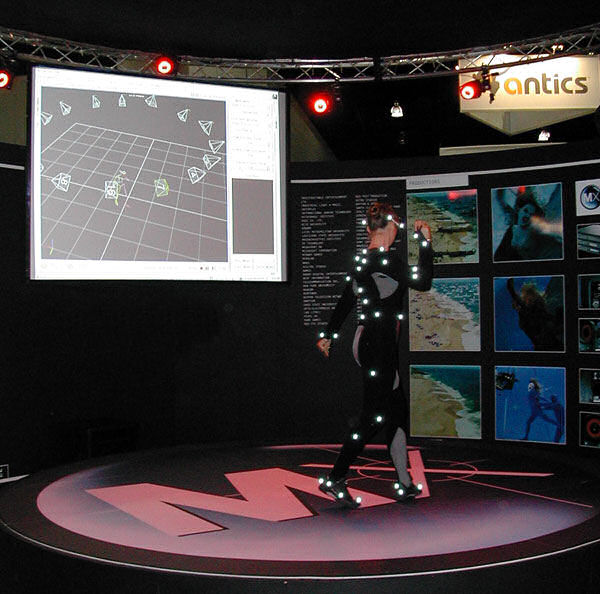
\includegraphics[width=5.5cm]{gfx/MotionCapture.jpg}}
	\subfigure[
		Two kinds of space balls and one space pilot.
	]{\label{FIG-SPACE-DEVICES}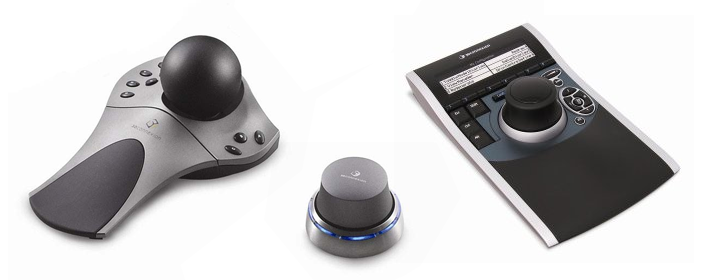
\includegraphics[width=6.5cm]{gfx/space-devices.png}}
	\caption{Interfaces}
\end{figure}

%\begin{figure}[!ht]
%	\centering
%	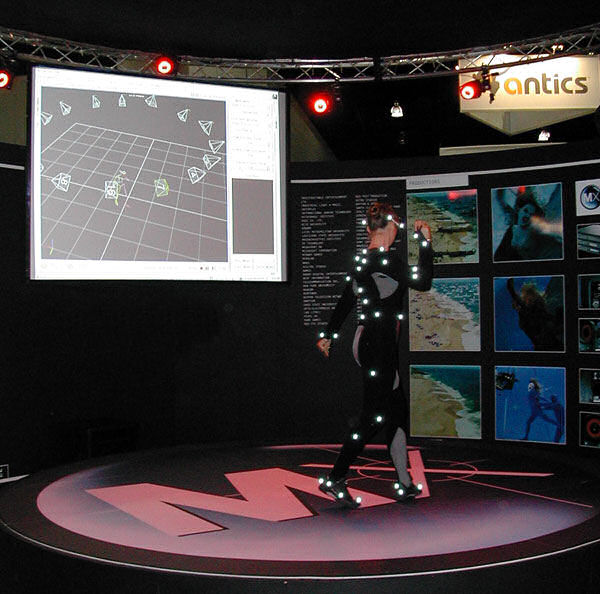
\includegraphics[width=6cm]{gfx/MotionCapture.jpg}
%	\caption{Motion tracking example:
%		the subject wears a suit with several markers distributed so that his skeleton
%		relative orientations can be reasoned.
%		An array of infrared cameras is rigged to the ceiling, reading marker positions.}
%	\label{FIG-MOTION-TRACKING}
%\end{figure}
%
%\begin{figure}[!ht]
%	\centering
%	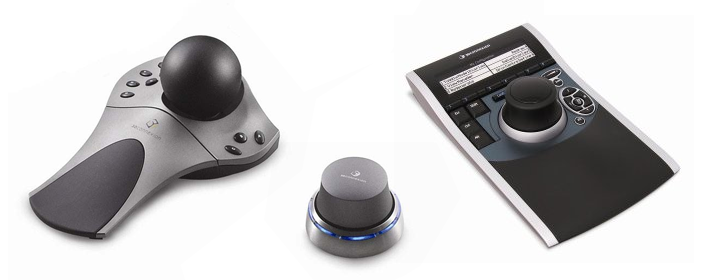
\includegraphics[width=8cm]{gfx/space-devices.png}
%	\caption{Two kinds of space balls and one space pilot.}
%	\label{FIG-SPACE-DEVICES}
%\end{figure}

The least intrusive interface would use speech recognition and either motion tracking or image processing,
the former being more driven to the purpose.
Speech recognition allows commands to be given to the system.
The remaining interface allows knowing positioning and rotation of users or parts of their bodies.
Tracking artifacts may either serve as a pointer or as a metaphor for direct manipulation.

\subsection{Sketching for Geometry Creation and Editing}

\subsubsection{Smart Sketchpad}
Wenyin et al. created Smart Sketchpad \cite{SMARTSK01}.
Smart Sketchpad recognizes standard shapes (rectangles, triangles, ellipses, straight lines)
and compound shapes such as arrowheads.

The article describes the steps necessary for shape recognition:
\begin{enumerate}
	\item Input as a chain of points;
	\item Polygonalize to polyline and refine endpoints;
	\item Close near endpoints. If closed go to step 6;
	\item If line ends near another line end, join them and go to step 3;
	\item Classify line as one of: straight line, polyline or free form curve. Go to step 8;
	\item Close shape recognition; *
	\item Estimate the parameter of the closed shape;
	\item Test if shape can be combined with other shapes in the drawing. If so repeat step 8, else end.
\end{enumerate}

The $6^{th}$ step was tested with both rule-based systems, support vector machines and neural networks.
The most successfully approach was SVN, with 97,5\% success, closely followed by NN.

\subsubsection{Assist}
Alvarado and Davis present a work towards an interface for mechanical designers named Assist \cite{FREEDOM01},
with the purpose of allowing them to sketch naturally and have the computer interpreting
their strokes into shapes like rods, hinges, polygons, etc.

The interpretation is a three stages procedure:

\begin{itemize}
	\item Match strokes to a series of templates;
	\item Rank interpretations with several heuristics about drawing style and mechanical engineering;
	\item Return the most consistent hypothesis.
\end{itemize}

Fig.\ref{FIG-FREEDOM01} illustrates the result.

The authors emphasize the difficulty they faced when replacing the original
human-made strokes by its computer interpretations.
Users prefer composing the whole drawing prior to computer interpretation replacement,
as opposed to a changeable estimation that refreshes at every added stroke.
Having the computer interpreting every stroke makes them feel they're losing control of the program. Even so, that was the path chosen by the authors because every extra stroke without giving feedback to the user increases the chance of misinterpretations.

Another relevant conclusion is that users expect symmetry to be kept regarding the interpreted
shapes, so it would be a good idea to detect and suggest alignment restrictions between shapes.

\begin{figure}[!ht]
	\centering
	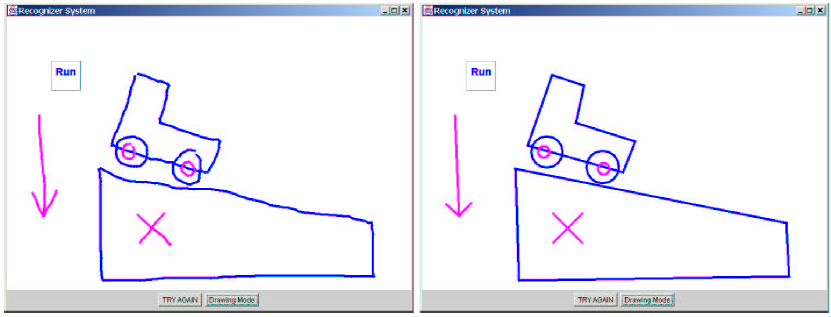
\includegraphics[width=11cm]{gfx/freedom01-1.png}
	\caption{Assist: A car on the hill. Drawn by the user (left), as interpreted and displayed (right).}
	\label{FIG-FREEDOM01}
\end{figure}

\subsubsection{Digital Clay}
Digital Clay \cite{DIGCLAY00} allows a user to draw freely and tries to convert the drawing into a 3D model.
See input and 3D result in Fig.\ref{FIG-DIGCLAY}.

It uses two techniques to achieve that:

\begin{itemize}
	\item The Huffman-Clowes algorithm, which identifies concave and convex vertices,
	requiring every line to connect to another line.
	The program additionally demands the object drawn to be solid;
	\item The 3D coordinates are inferred based on inherent rules
	that govern each type of drawing projection.
	Examples of applied rules:
	\begin{itemize}
		\item Axes of isometric drawings have equal angles between them;
		\item Perspective drawings show foreshortening of lines as we get closer to the viewer.
	\end{itemize}
\end{itemize}

The downfalls of this method are
the impossibility of describing occluded faces and
the limited editing capacities available once the conversion has been done.

\begin{figure}[!ht]
	\centering
	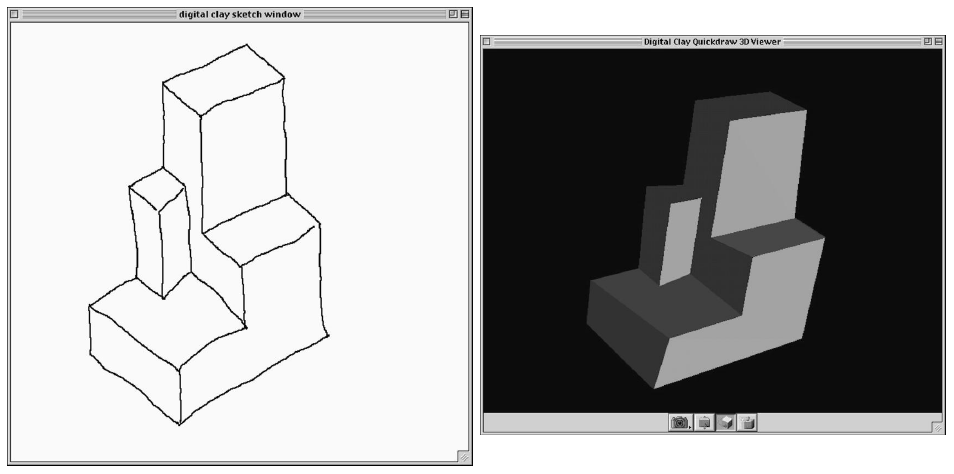
\includegraphics[width=11cm]{gfx/digclay00-1.png}
	\caption{Digital Clay: Raw sketch input and its 3D interpretation.}
	\label{FIG-DIGCLAY}
\end{figure}

\subsubsection{Discussion}

In \cite{SMARTSK01} a useful comparison between alternative implementations of their
shape recognition algorithm is performed.
Wenyin at al. conclude in their paper that Support Vector Machines are the faster implementation.
The proposed algorithm itself is relatively simple and may be generalized to 3D shapes.

The method proposed by Alvarado and Davis in \cite{FREEDOM01} works nicely but has applications
only in 2D space.
Additionally, users felt uneasy as the geometric shapes they drawn kept continuously being
replaced by the computer program, making them feel having lost control of the application.

Schweikardt and Gross \cite{DIGCLAY00} developed the only system discussed here that allows 3D drawing.
Though its results are interesting, it shouldn't be used because it only allows describing part
of geometry (the occluded geometry is undefined) and because it doesn't allow successive
iterations to fill in the undefined geometry.

\subsection{Helping the User: Suggested Constraints}

\subsubsection{Pegasus}
Igarashi and Hinckley present a 2D sketching system named Pegasus \cite{BEAUTY97}.
It receives user strokes and converts them, generating candidates by taking into
account restrictions for:
vertex connection, segment connection, parallelism, perpendicularity,
alignment, congruence, symmetry and interval equality.

The application presents the most relevant candidates to the user and highlights
the highest relevant one.
The user can either accept it or select another candidate by tapping on it as seen
in Fig.\ref{FIG-PEGASUS}.

\begin{figure}[!ht]
	\centering
	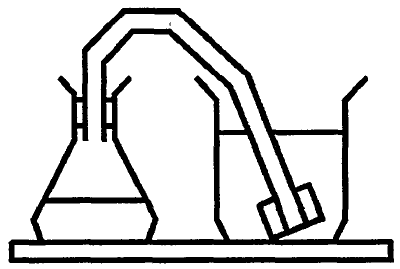
\includegraphics[width=5cm]{gfx/beauty97-1.png}
	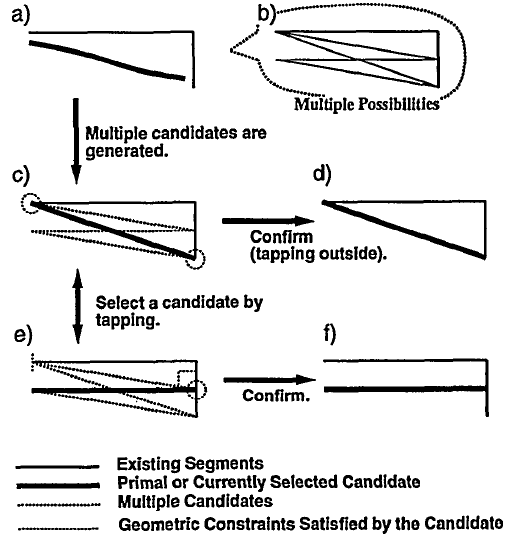
\includegraphics[width=5.5cm]{gfx/beauty97-2.png}
	\caption{Pegasus: A diagram drawn on Pegasus without using any editing commands such as rotation,
		copy or griding (left); interaction with multiple candidates (right).}
	\label{FIG-PEGASUS}
\end{figure}

\subsubsection{Discussion}

Igarashi at al. present in \cite{BEAUTY97} a useful way of aiding the user.
Most elements in architecture subsume to these constraints.
Applying a technique of this kind gains more relevance in
the 3D architecture problem because users will be modeling in 3D.
Humans are more prone to drawing errors in a task like this,
benefiting more from beautification algorithms.

\subsection{Navigation}

\subsubsection{Smart and Physically Based Navigation}
In order to ensure users not ``getting lost'' in the virtual space,
Buchholz, Bohnet and D�llner \cite{SMARTCAM05}
propose a camera that is is both smart and physically-based.
It is smart in the sense that it is aware of confusing,
disorienting viewing situations, providing means to circumvent them.
It is physically based because it is supported by a physically based model of 3D motion
to ensure steady, continuous user movements.

In order to solve the disorientation problem, the camera must identify situations
when to intervene.
For that matter a metric, called orientation value, was created.
Each view is classified by counting its pixels, granting each one a different value:
landmarks are granted the highest values; terrain gets high values and sky gets low values.
A threshold can then be established and views below it are classified ``disoriented''.

When such an event takes place, smart navigation techniques restrict camera control.
The constraints posed to user control must be as comprehensible as possible.
Camera movement should also be time-coherent and physically sound.

The maintenance strategy solves critical situations such as (see Fig.\ref{FIG-SMARTCAM1}, left):

\begin{enumerate}[a)]
	\item The user rotates the flight direction and causes the camera to look too far beyond the terrain border.
		The rotation is accepted but outweighed by a slight rear movement away from the border.
	\item The user is flying forward beyond the terrain border.
		The maintenance strategy temporarily tilts down the view direction until a maximum angle is reached.
	\item If no more tilting is possible, the strategy rotates the flight direction parallel to the terrain
		to fly along the terrain border.
\end{enumerate}

\begin{figure}[!ht]
	\centering
	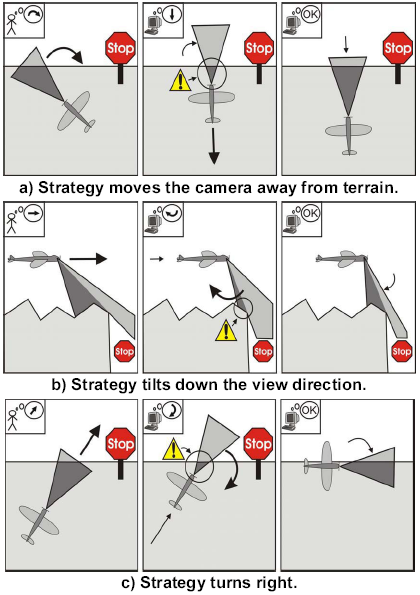
\includegraphics[height=7cm]{gfx/smartcam05-1.png}
	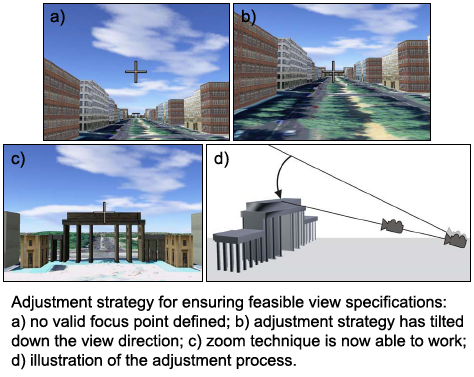
\includegraphics[height=5cm]{gfx/smartcam05-2.png}
	\caption{SPB Cam: Maintenance strategy for keeping high orientation values (left); Adjustment strategy for ensuring of feasible view specifications (right).}
	\label{FIG-SMARTCAM1}
\end{figure}


%\subsubsection{}

%\cite{SKAN02}
%\cite{DESFUT04}

